% !TeX encoding = UTF-8
% !TeX program = pdflatex
% !BIB program = bibtex

%%% Um einen Artikel auf deutsch zu schreiben, genügt es die Klasse ohne
%%% Parameter zu laden.
\documentclass[english]{lni}
%\documentclass[a4paper,pagesize,13pt,normalheadings,DIV=10]{scrarticle}
\usepackage{graphicx}
%\usepackage[caption=false]{subfig}
\newcommand{\TODO}[1]{\colorbox{yellow}{#1}}
\usepackage{amsfonts}
\usepackage{amsthm}
\usepackage{mathtools}
\usepackage{paralist}

% Figures
\usepackage{caption}
\usepackage{subcaption}

% Algorithms
\usepackage{algorithm}
\usepackage[noend]{algpseudocode}
\theoremstyle{definition}
\newtheorem{definition}{Definition}[section]

% Tables
\usepackage{booktabs}

\newcommand{\sql}[1]{\texttt{#1}}

%%% To write an article in English, please use the option ``english'' in order
%%% to get the correct hyphenation patterns and terms.
%%% \documentclass[english]{class}
%%
\begin{document}
%%% Mehrere Autoren werden durch \and voneinander getrennt.
%%% Die Fußnote enthält die Adresse sowie eine E-Mail-Adresse.
%%% Das optionale Argument (sofern angegeben) wird für die Kopfzeile verwendet.
\title[PostBOUND]{PostBOUND: PostgreSQL with Upper Bound SPJ Query Optimization }
%%%\subtitle{Untertitel / Subtitle} % if needed
\author[Rico Bergmann et al.]
{Rico Bergmann\footnote{Technische Universit\"at Dresden, Database Research Group, 01062 Dresden,
Germany,\newline \email{{rico.bergmann1,axel.hertzschuch,claudio.hartmann,dirk.habich,wolfgang.lehner}@tu-dresden.de}} \and
Axel Hertzschuch$^1$ \and
Claudio Hartmann$^1$ \and
Dirk Habich$^1$ \and
Wolfgang Lehner$^1$}
\startpage{1} % Beginn der Seitenzählung für diesen Beitrag / Start page
\editor{B. K{\"o}nig-Ries et al.} % Names of Editors
\booktitle{Datenbanksysteme f{\"u}r Business, Technologie und Web (BTW 2023)} % Name of book title
\yearofpublication{2023}
%%%\lnidoi{18.18420/provided-by-editor-02} % if known
\maketitle

\begin{abstract}
A variety of query optimization papers have shown the disastrous effect of poor cardinality estimates on the overall runtime for arbitrary select-project-join (SPJ) queries.
Especially, underestimating join cardinalities for multi-joins can lead to catastrophic join orderings.
A promising solution to overcome this problem is query optimization based on upper bounds for the join cardinalities.
In this domain, our proposed UES concept is presently the most efficient technique featuring a simple, yet effective upper bound for an arbitrary number of joins.
To foster research in that direction, we introduce \emph{PostBOUND}, our generalized framework to seamlessly integrate upper bound SPJ query optimization in PostgreSQL.
\emph{PostBOUND} provides abstractions to calculate arbitrary upper bounds, to model joins required by an SPJ query and to iteratively construct an optimized join order.
To highlight the extensibility of \emph{PostBOUND}, and to show the research potential, we additionally present two tighter upper bound UES variants using top-k statistics in this paper.
In our evaluation, we show the efficiency and applicability of \emph{PostBOUND} on different workloads as well as using different PostgreSQL versions. 
Additionally, we evaluate both presented tighter upper bound variant ideas.
\end{abstract}



\begin{keywords}
SPJ queries \and join order \and join cardinalities \and upper bound \and generalization %Keyword1 \and Keyword2
\end{keywords}
%%% Beginn des Artikeltexts
%\chapter{Related Work}
%\label{chap:related-work}

\section{Introduction}
\label{sec:Introduction}

The optimization of arbitrary select-project-join (SPJ) queries is still an open research topic and far from being solved~\cite{DBLP:journals/pvldb/LeisGMBK015}.
For example, one of the most challenging and open issues for complex SPJ queries is finding a good join order~\cite{DBLP:conf/sigmod/CaiBS19,hertzschuch-21-ues,DBLP:journals/pvldb/LeisGMBK015}.
To tackle this issue, the majority of existing approaches requires reliable precise cardinality estimates for arbitrary joins including joins over intermediate join results and pre-filtered base tables.
To provide these reliable estimates, traditional techniques frequently rely on basic heuristics that may assume predicate independence and a uniform distribution of attribute values~\cite{DBLP:journals/pvldb/LeisGMBK015}. 
However, relying on these assumptions can lead to disastrous join orderings~\cite{DBLP:journals/pvldb/LeisGMBK015}. 
Thus, various sophisticated techniques for the join cardinality estimation have been proposed in recent years.
On the one hand, sampling approaches seem appealing~\cite{DBLP:conf/cidr/LeisRGK017,DBLP:conf/cidr/MoerkotteH20,DBLP:conf/sigmod/ZhaoC0HY18}, but they do not scale well to many joins~\cite{DBLP:conf/sigmod/ChenY17,DBLP:conf/sigmod/ZhaoC0HY18}. 
On the other hand, modern estimation approaches rely on machine learning techniques~\cite{DBLP:conf/cidr/KipfKRLBK19,DBLP:conf/sigmod/WoltmannHTHL19} as they are able to model complex data characteristics. 
However, these ML approaches do not yet cover all relevant filter predicate types and their training depends on executing a plethora of joins, which may take days or weeks~\cite{DBLP:conf/sigmod/WoltmannHHL20,DBLP:conf/btw/WoltmannHHL21}.

\begin{figure}[t]
    \centering
    \includegraphics[width=0.7\linewidth]{figures/plot-ues-overestimation.pdf}
    \caption{Upper bound overestimation of UES for the Join-Order-Benchmark.}
    \label{fig:UESOverestimationJOB}
    \vspace{-0.4cm}
\end{figure}

Thus, state-of-the-art approaches to find good join orders based on reliable cardinality estimates do not seem to be the right way.
In contrast to that, approaches using guaranteed upper bounds for join cardinalities is a very promising alternative leading to better and more robust join ordering for complex SPJ queries~\cite{DBLP:conf/sigmod/CaiBS19,DBLP:journals/corr/abs-2201-04166,hertzschuch-21-ues}. 
In that direction, we have recently introduced a novel concept called \emph{UES}~\cite{hertzschuch-21-ues}. 
The most outstanding feature of ~\emph{UES} is its simplicity, achieved by three building blocks:
\begin{compactitem}
\item[\emph{U}-Block:] Assuming only basic attribute statistics and accurate selectivity estimates for filters over base tables, we defined a simple, yet effective \textbf{U}pper bound for an arbitrary number of joins. In particular, our \emph{UES} upper bound calculates the worst-case cardinality using only the maximum value frequency per join attribute. 
\item[\emph{E}-Block:] Appropriately \textbf{E}numerating joins according to our upper bound effectively prevents overly aggressive (sometimes disastrous) join orderings.
\item[\emph{S}-Block:] To guarantee accurate selectivity estimates even for complex filters in SPJ-queries required by the \textbf{U}-Block, we treat \textbf{S}ampling like query execution.
\end{compactitem}

\textbf{Our Contributions:} 
In this paper, we introduce \emph{PostBOUND}, our generalized framework implementation around the general \emph{UES} concept making upper bound SPJ query optimization a first class citizen in PostgreSQL. 
\emph{PostBOUND} provides abstractions to integrate arbitrary upper bounds for join cardinalities, to model joins required by a query and to determine an optimized join order.
These abstractions are supplemented by a customized version of the UES algorithm and accompanied by other assisting components such as estimation strategies for base table filters or an infrastructure for physical operator selection.
Moreover, our overall framework is implemented in Python and it is designed for extensibility.% to advance research in this context.% through a comprehensive and extensible system.

To demonstrate this extensibility and to show ongoing research potential, we additionally introduce two tighter upper bound variant ideas as a generalization of UES. 
Fig.~\ref{fig:UESOverestimationJOB} exemplary illustrates the overestimation factor of the UES upper bound compared to the real query results for the \emph{Join-Order-Benchmark (JOB)}~\cite{DBLP:journals/pvldb/LeisGMBK015}.
It is clearly visible that the overestimation in the range from $10^3$ to $10^{16}$ is extreme leading to a very pessimistic approach. 
One of the disadvantages of this high overestimation is that the determined join order for a SPJ query could be too defensive and there could be a join order providing a faster run time. 
Another disadvantage is that the upper bound cannot be used for the physical operator selection~\cite{hertzschuch-21-ues,DBLP:journals/pvldb/HertzschuchHHL22}. 
Thus, an obvious optimization opportunity of our \emph{UES} approach is to compute tighter upper bounds to overcome these disadvantages.
 
\textbf{Contributions in Detail and Outline:} To summarize, we make the following contributions defining also the outline of this paper:
\begin{compactitem}
\item In Section~\ref{sec:UES}, we recap our \emph{UES} concept as foundation for the remainder of the paper.
\item Our developed PostgreSQL extension called \emph{PostBOUND}\footnote{We will make \emph{PostBOUND} available open-source in
time for BTW 2023 and we would happily join the reproducibility effort of BTW 2023.} is described in Section~\ref{sec:PostBound}. \emph{PostBOUND} makes upper bound SPJ query optimization a first class citizen in PostgreSQL and \emph{PostBOUND} is designed as extensible framework.% to foster research in that direction.
\item We enhance the \emph{UES} concept with an idea for a generalized approach to tighten our upper bound based on top-k statistics in Section~\ref{sec:TighterBounds}. 
\item Section~\ref{sec:Eval} presents selective results of our comprehensive evaluation. In particular, we focus on the evaluation (i) of the upper bound optimization on different workloads as well as different PostgreSQL versions and (ii) of the impact of the tighter bounds.  
\end{compactitem}
Finally, we close the paper with related work in Section~\ref{sec:RealtedWork} before concluding in Section~\ref{sec:Conclusion}. 


%As shown in~\cite{}, our \emph{UES} concept outperforms other existing upper bound as well as traditional approaches even though our worst-case upper bound overestimates the real cardinalities by large factors. 







%%\begin{itemize}
%    \item some nice introduction why we need this paper
%    \item paper contributes a framework for the UES algorithm
%    \item framework allows the evaluation of various upper bounds, query execution plan shapes, filter selectivity estimators, etc. in the context of the general UES strategy. 
%\end{itemize}
\section{UES - Join Ordering with Simple Upper Bound}
\label{sec:UES}

In contrast to state-of-the-art approaches (see Section~\ref{sec:RealtedWork}), our UES concept~\cite{hertzschuch-21-ues} follows a completely different idea to determine good join orderings for SPJ queries: instead of trying to obtain precise estimates for join cardinalities, it calculates theoretical upper bounds of the sizes of intermediate result sets and uses these bounds in a heuristic join enumeration algorithm. 
This concept is based on the insight that the duration of query workloads is often dominated by the runtime of very few queries that take an exceptionally long amount of time. 
Meanwhile, most queries in a typical workload can be answered rather quickly. 
This phenomena is referred to as \emph{tail latency}.
Thus, a novel query optimization strategy should focus on improving these long-running queries, instead of speeding up queries that are already fast. 
However, this can usually not be achieved by improving the runtime in the average case, since new outliers can become part of the tail latencies. 
In contrast, a correct theoretical upper bound can never be wrong in the sense that the true cardinalities exceed the bound. 
By feeding these worst-case estimates to the join enumeration algorithm, it will probably choose a join order that is too pessimistic in the sense that another join order could have provided a faster runtime. 
But it will never choose a join order that is too optimistic, i.e. a plan that only works if the intermediate cardinalities are indeed small and takes a much longer time to execute if this hope is not met. Following this general philosophy of focusing on the long running queries, it is acceptable if very fast queries get slightly slower, as long as the tail latencies are removed. In the following, we sketch both the upper bounds for join cardinalities, as well as the heuristic join enumeration algorithm of UES.

Our UES upper bounds of join intermediate cardinalities are estimated via most frequent value statistics on the join columns. In fact, the only metadata necessary to calculate upper bounds with UES are the frequencies of the most common values of the join attributes and the total number of (filtered) tuples per base table. These statistics are then combined with a number of pessimistic assumptions regarding the distribution and correlation of the attribute values.
For brevity the calculation is only summarized here, since the final formula is already presented and justified in~\cite{hertzschuch-21-ues}.
To estimate the size of a join $R.x \bowtie S.y$ on (filtered) base tables $R$ and $S$ while only using the most frequent values for $R.x$ and $S.y$, a first pessimistic assumption is used: the attributes are \emph{assumed} to be uniformly distributed, with the maximum value frequency (MF) therefore also being the only frequency shared by all values. 
Based on these frequencies and the total number of tuples per (filtered) relation ($|\sigma(R.x)|, |\sigma(S.y)|$), the minimum number of distinct values per attribute can be estimated as $|\sigma(R)| / MF(R.x)$ for $R$ and likewise for $S$.
To combine these per-table values into an estimate for their join result, a second pessimistic assumption is used: the attribute values are \emph{assumed} to overlap perfectly, i.e. each value in $R.x$ has a matching join partner in $S.y$ and vice-versa. 
This leads to $MF(R.x) \cdot MF(S.y)$ many outgoing tuples per value combination due to the uniformity assumption. 
Since there are at most $min(|\sigma(R.x)| / MF(R.x), |\sigma(S.y)| / MF(S.y))$ many such combinations, the upper bound can be calculated as
$$upper(|\sigma(R) \bowtie \sigma(S)|) := min\Bigl(\frac{|\sigma(R)|}{MF(R.x)}, \frac{|\sigma(S)|}{MF(S.y)}\Bigr) \cdot MF(R.x) \cdot MF(S.y)$$

\begin{figure}[t]
    \centering
    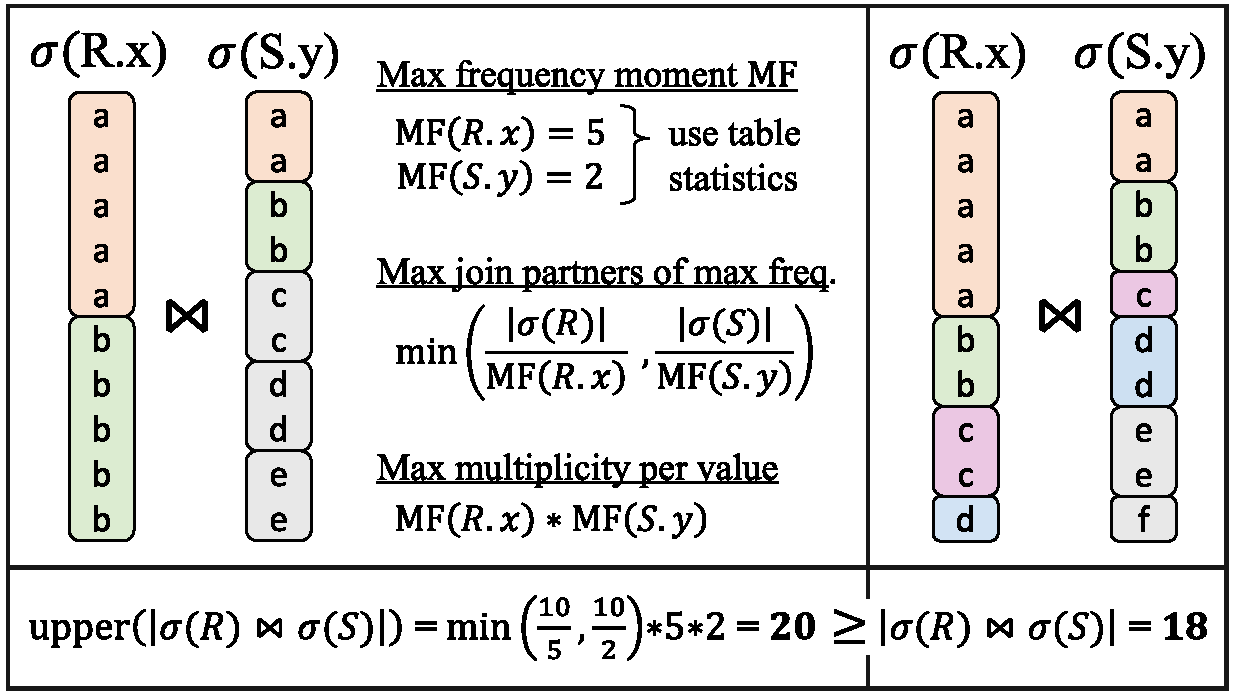
\includegraphics[width=0.7\linewidth]{figures/upperBoundExplV6_.pdf}
    \caption{Illustration of the UES upper bound (taken from \cite{hertzschuch-21-ues}).}
    \label{fig:upperBoundExpl}
\end{figure}

Fig.~\ref{fig:upperBoundExpl} illustrates our UES upper bound concept, using an example. 
The left-hand side depicts the worst-case -- used to derive the upper bound -- constrained by the table statistics, while the right-hand side depicts the actual join.
Note that $R$ and $S$ do not need to be base tables. 
Instead they can be the result of some other join just as well. 
For example, without loss of generality, we can assume that $R = R_1 \bowtie_{R_1.x = R_2.y} R_2$. 
In this case, $|\sigma(R)| = upper(|R_1 \bowtie R_2|)$ and $MF(R.x) = MF(R_1.x) \cdot MF(R_2.y)$. 
This enables the calculation of upper bounds for any join in a recursive manner. 
One central downside of this approach is the propagation of errors, in this case of overestimated result sizes. 
Since the estimation of an $n$-way join requires estimates of $n-1$ smaller joins building on top of each other, estimates grow larger and larger as already shown in Fig.~\ref{fig:UESOverestimationJOB}.
%This puts special emphasis on the importance of tight upper bounds. 

Based on this upper bound for join cardinalities, the join order in UES is obtained using a heuristic algorithm~\cite{hertzschuch-21-ues}.
The UES join enumeration algorithm tries to choose each join such that the sizes of intermediate results are minimized in each step. 
To make this choice, the upper bounds of candidate joins are calculated and the join with smallest bound is executed. 
However, this process is only applied to n:m joins. 
Primary key/foreign key joins (P/K joins) are greedily included as soon as possible. 
This strategy is justified by a central property of P/K joins: When the foreign key partner is already present in the intermediate result, joining the primary key table may only reduce but never expand the size of the intermediate result. In this sense, P/K joins act as special filters. 
To facilitate this filtering property even further, a P/K join can be executed as a subquery: suppose an (intermediate) table $\Tilde{T}$ should be joined with a foreign key table $T_{FK}$, which in turn has to be joined with a Primary Key table $T_{PK}$. 
The canonical way of executing this join would be $(\Tilde{T} \bowtie T_{FK}) \bowtie T_{PK}$. The n:m join $\Tilde{T} \bowtie T_{FK}$ would most likely (i.e. following the pessimistic assumption) increase the size of the intermediate result. 
Afterwards, joining $T_{PK}$ could potentially reduce the size of the intermediate result again. 
If such a reduction is guaranteed, executing $T' := T_{FK} \bowtie T_{PK}$ first and afterwards $\Tilde{T} \bowtie T'$ would minimize work for the second join. Thus, when choosing the next n:m join to execute, UES tries to pre-filter the join partners via P/K joins. 
If this does not guarantee a smaller intermediate result, the Primary Key partner will be joined after the n:m join has been executed. To some extent, this strategy resembles the well-known pushdown of filter predicates.

To better illustrate the concept of P/K filters, consider part of query 8d of the JOB: \sql{SELECT * FROM cast\_info ci, company\_name cn, movie\_companies mc WHERE cn.country\_code = '[us]' AND mc.company\_id = cn.id AND ci.movie\_id = mc.movie\_id}. Overall, this query fragment produces about 59 million result tuples. It contains one P/K join between \sql{movie\_companies} and \sql{company\_name} and one n:m join between \sql{cast\_name} and \sql{movie\_companies}. In this case, the P/K join $mc \bowtie cn$ reduces the cardinality of \sql{movie\_companies} from about 5 million to 2 million. This essentially halves the work for the following n:m join between \sql{cast\_name} and \sql{movie\_companies}, since \sql{company\_name} ``filtered'' its P/K partner.

\section{PostBOUND - PostgreSQL Extension}
\label{sec:PostBound}

\begin{figure}[tb]
	\centering
	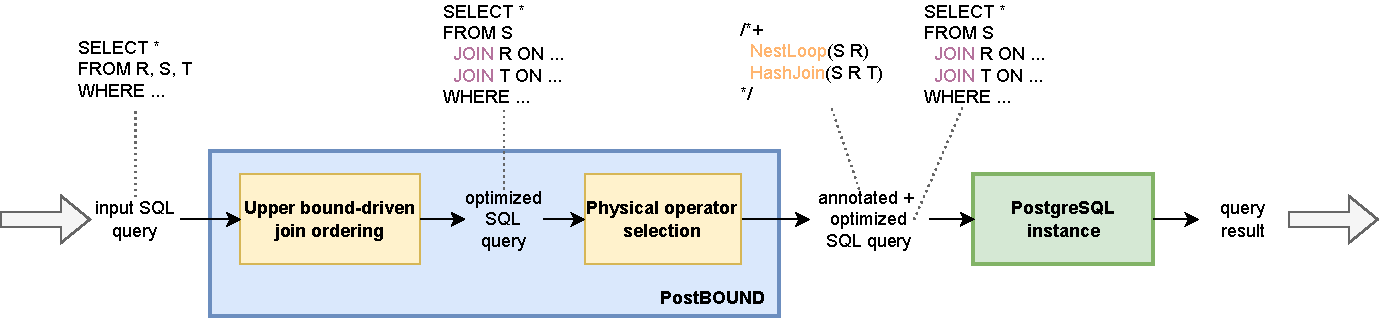
\includegraphics[width=0.95\linewidth]{figures/postbound-workflow-rework.pdf}
	\caption{The basic \emph{PostBOUND} query optimization workflow.}
	\label{fig:postbound-workflow}
\end{figure}

In this section, we present \emph{PostBOUND}, our developed framework to seamlessly integrate upper bound-driven optimization of SPJ queries into PostgreSQL.
At its core, \emph{PostBOUND} consists of two components as depicted in Fig.~\ref{fig:postbound-workflow}, which are completely implemented in Python: 
First, for each incoming SQL query, the \texttt{join ordering component} determines an optimized join order that is used for query execution. 
The underlying process applies a generalized and extensible implementation of our UES concept (see Section~\ref{sec:UES}). 
The output of this first component is a rewritten SQL query with an explicit join order.
Secondly, our subsequent \texttt{physical operator selection} component enforces the usage of individual physical join and base table scan operators. 
The resulting query annotations to enforce physical operators are used together with the rewritten SQL of our first component to execute the query with an arbitrary PostgreSQL instance.
With this approach, the join order as well as the physical operator selections are fixed by \emph{PostBOUND} using an upper bound-driven optimization concept. 
Implementation details of both components are described in the following sections\footnote{ 
Although \emph{PostBOUND} is currently tailored to PostgreSQL, it can be adapted to other database systems and we plan to integrate different backends in the near future.}.

\subsection{Upper Bound-driven Join Ordering Component}
\label{sec:postbound-join-ordering}


The upper bound-driven join ordering is the first component of \emph{PostBOUND} and it focuses on a robust join sequence in order to prevent disastrous execution plans.
The main goal of this component is to optimize the join order of an arbitrary SQL query by transforming implicit joins like \sql{SELECT * FROM R, S, T WHERE ...} into an explicit ordering via \sql{JOIN} clauses, such as \sql{SELECT * FROM S JOIN R ON ... JOIN T ON ...}. During query execution, PostgreSQL provides means to enforce such an ordering of \sql{JOIN} statements.
Fig.~\ref{fig:postbound-interaction} shows the general steps involved in this process:
First, a \emph{join graph} is constructed by parsing the incoming SQL query.
This graph serves as the central data structure for optimization and describes the role each table plays in the query. 
We apply the same distinction between n:m joined tables and primary key joined tables, as originally proposed in UES~\cite{hertzschuch-21-ues}.
Based on this graph, the actual optimization loop is executed in the \texttt{join graph enumerator}. 
During each iteration, the algorithm pulls n:m candidate tables from the join graph and evaluates their current upper bounds, such that the candidate with minimum bound is inserted into the join tree (tables colored in orange in Fig.~\ref{fig:postbound-interaction}).
This selection focuses only on n:m joined tables, because primary key/foreign joins are again treated as special filters of the foreign key (and by extension n:m joined) table that can potentially lower the candidate's upper bound.
Therefore, primary key tables are inserted into the join tree together with their foreign key counterpart. 
Again, following the UES philosophy, the join between the candidate table and its primary key partners can be executed as a subquery, as the enumerator sees fit (see below for details).
Once all tables of the join graph have been included in the join tree, the rewritten query with an explicit join order syntax is constructed based on the derived optimal join order.

\begin{figure}[tb]
	\centering
	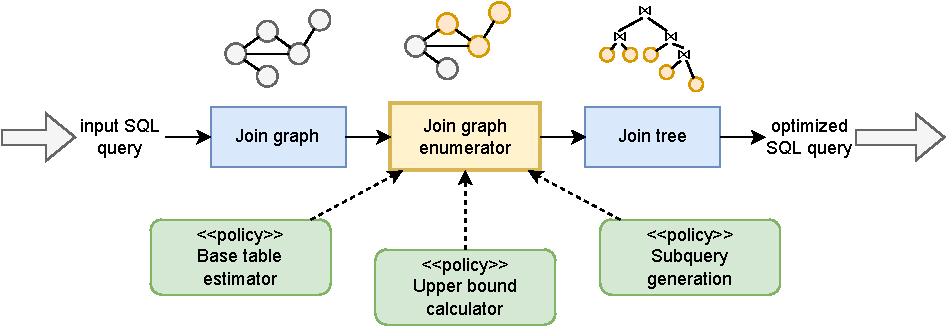
\includegraphics[width=0.95\linewidth]{figures/postbound-interaction-rework.pdf}
	\caption{Interaction between the core \emph{PostBOUND} components for join ordering.}
	\label{fig:postbound-interaction}
\end{figure}

In \emph{PostBOUND} we expand on the original UES algorithm in two ways: On the one hand, this entire enumeration process can be adapted with custom policies to modify specific aspects of its behavior. These policies include:

\begin{compactitem}
    \item[\textbf{Base table estimates:}] The \texttt{join ordering} component of \emph{PostBOUND} does not require a specific strategy to estimate the number of tuples in a (filtered) base table. It only relies on the existence of a numerical estimate and makes no assumption about how it is obtained. Nevertheless, three basic strategies are already provided and new strategies can be injected easily. The provided strategies include: (i) delegating the estimation process to the PostgreSQL-native optimizer, (ii) sampling a fraction of the filtered table, or (iii) executing the entire filter predicate and counting the result tuples.
    \item[\textbf{Upper bound calculation and statistics:}] To obtain upper bounds of join cardinalities, different strategies have been proposed in recent literature~\cite{DBLP:conf/sigmod/CaiBS19,DBLP:journals/corr/abs-2201-04166,hertzschuch-21-ues}. \emph{PostBOUND} does not restrict the choice of any particular formula, as long as it is capable of the calculation of an upper bound of any $n$-ary join. Currently, the UES formula (see Section~\ref{sec:UES}) and two variations (see Section~\ref{sec:TighterBounds}) are provided with \emph{PostBOUND}. Since join upper bound calculation oftentimes relies on specific \emph{statistical information}, each calculation strategy ships its own tailored implementation. The statistics interface receives update information from the optimization loop.
    \item[\textbf{Subquery generation:}] \label{item:postbound-subqueries} Lastly, the \texttt{join ordering} component of \emph{PostBOUND} also delegates the decision when to generate subqueries for primary key/foreign key joins to custom policies. In this case, four strategies are already supplied by default: (i) a greedy strategy that always generates subqueries, (ii) a defensive strategy that generates subqueries if they guarantee to reduce the size of the foreign key table (as proposed in \cite{hertzschuch-21-ues}), (iii) a ``smart'' strategy that generates subqueries if a reduction below a certain threshold is guaranteed (which is a generalization of strategy (ii)), and finally, (iv) a strategy that never generates subqueries at all, thereby leaving all join paths linear.
\end{compactitem}

On the other hand, the entire enumeration process is mainly tailored to SPJ queries containing a mixture of n:m and primary key/foreign key joins. 
To broaden this scope, if an incoming SQL query does not match this structure, it will be handled by specialized procedures:

\begin{compactitem}
    \item[\textbf{Primary key/foreign key queries:}] To optimize queries that do not contain any n:m join -- such as queries on star- or snowflake schemas -- a heuristic approach inspired by UES is used. In this case and since primary key/foreign key joins are bound to never produce more tuples than the cardinality of the foreign key relation, our enumeration algorithm starts with the smallest foreign key table and iteratively includes connected tables according to their respective cardinality estimates. This strategy tries to minimize the number of tuples that have to be processed, but only treats the join order as a local optimization problem. An extension that also considers the join cardinalities could be a natural and effective improvement in future work.
    \item[\textbf{Cross product queries:}] Queries with cross products are characterized by tables that are neither directly nor indirectly linked with join predicates. Using the join graph, this situation can be easily detected through the existence of multiple graph components. Since each of these components represents a complete join graph on its own, an optimized upper bound-driven join order can be obtained per partition. Afterwards, a final join order can be constructed by sorting the individual join trees according to their upper bounds.
    \item[\textbf{Composite join predicates:}] In contrast to the two previous extensions, composite join predicates do not influence the join order itself. Rather, composite join predicates need to be handled during the upper bound calculation and are, thus, subject to the policies. However, they still constitute a special case that needs to be considered to ensure independence from specific workloads. Therefore, they are quickly discussed here. For upper bound-driven calculation, composite join predicates can be handled quite naturally: Since a conjunctive predicate requires each of the individual base predicates to be fulfilled, the final upper bound is constrained by the smallest estimate of the base predicates. Thus, the upper bound approach can simply calculate the minimum of base estimates. Other upper bound approaches may rely on different strategies such as the calculation of mean bounds, but for UES as well as the two presented variants in Section~\ref{sec:TighterBounds}, the minimum strategy is used.
\end{compactitem}

Based on these extensions, \emph{PostBOUND} is currently capable of optimizing SPJ queries, as well as some non-SPJ queries, as long as the following requirements are met: (i) each part of the \sql{SELECT} clause is either directly derived from a base attribute or an aggregation of such attributes, (ii) all joins are either equality predicates over base table attributes, or conjunctions of such predicates, (iii) each base table can optionally be filtered using arbitrary predicates that are not optimized further, and (iv) each query can optionally contain a \sql{GROUP BY}, \sql{ORDER BY}, or \sql{HAVING} clause, which are also ignored during optimization. These restrictions are mostly due to technical reasons to keep the implementation effort manageable, rather than being caused by limitations of the underlying ideas.


\subsection{Physical operator selection component}
\label{sec:postbound-operator-selection}

For an efficient query execution, not only the join order is important, but also the selection of the best-fitting physical operators~\cite{DBLP:journals/pvldb/HertzschuchHHL22}. 
In \emph{PostBOUND}, this selection process is handled by a dedicated \texttt{physical operator selection} component (cf. Fig.~\ref{fig:postbound-workflow}). 
Although many state-of-the-art query optimizers intertwine the operator selection and the determination of the optimal join order, the upper bound approach makes this difficult due to the overestimation as shown in Fig.~\ref{fig:UESOverestimationJOB}. Therefore, new, specific approaches are required. 
In~\cite{DBLP:journals/pvldb/HertzschuchHHL22}, we have recently presented such a selection approach using a learning-based concept that allows physical operator decisions for arbitrary join paths based on learned query feedback.
Other approaches are also conceivable and thus, we decided to provide a specific component in \emph{PostBOUND} to accommodate such selection approaches. 

Since forcing the execution of joins or table scans with specific algorithms depends strongly on the concrete database system, \emph{PostBOUND} focuses on two means supported by PostgreSQL. 
The first strategy uses runtime variables that modify the behavior of the PostgreSQL planner. 
For example, the \mbox{\sql{SET enable\_nestloop = 'off';}} option used by UES disables nested loop joins globally for all following queries in a workload. 
Secondly, \emph{PostBOUND} also provides interfaces that force individual joins to be executed with specific operators. 
This feature is based on the \emph{pg\_hint\_plan}\footnote{\url{https://github.com/ossc-db/pg_hint_plan/}} extension that specifies a number of \emph{query hints}. 
A hint is essentially a comment preceding an SQL query that modifies the execution and optimization behavior of PostgresSQL for that specific query. 
For example, the hint \sql{/*+ HashJoin(movies actors) */} would enforce the join between \sql{movies} and \sql{actors} to be executed by a Hash join. 
How these hints are generated is left to user-specific selection strategies. 
In our ongoing research, we want to generate query hints for joins based on upper bounds, which however requires tighter upper bounds. One approach to infer such bounds is presented in the following section.

%\subsection{Summary}
%\label{sec:postbound-summary}

%\emph{PostBOUND} is our framework to systematically evaluate different approaches to pessimistic query optimization. \emph{PostBOUND} is a PostgreSQL-specific set of components that use a query optimization algorithm inspired by UES. The algorithm enables the adaption of base table estimates, join cardinality estimates and the generation of subqueries. Furthermore, \emph{PostBOUND} is designed to operate without any additional user-supplied data and fetches all required information from the Postgres instance. This enables independence from specific benchmarks and database schemas. Using this framework, we can optimize different workloads and compare their results in a reproducible and transparent way.

\section{Towards Tighter Upper Bounds with Top-K Lists}
\label{sec:TighterBounds}

%Upper bounds are attractive for query optimization because they provide robustness: By preparing the query execution plan for the worst possible scenario, the database system can never produce overly optimistic plans that lead to catastrophic regressions. If however the calculated upper bounds overestimate the actual cardinalities by a large margin, plans may become too defensive and refrain from using operators and join orders that work best on small amounts of tuples. This in turn may lead to slower queries. To circumvent this issue, we explore means to tighten the UES upper bounds while still relying on basic table statistics.

As presented in the previous section, \emph{PostBOUND} is a novel framework for upper bound-driven query optimization of SPJ queries based on a generalized version of the UES concept~\cite{hertzschuch-21-ues}. 
Since the original UES algorithm only calculates upper bounds based on the most frequent attribute value~\cite{hertzschuch-21-ues}, this upper bound approach highly overestimates the join intermediate cardinalities (cf. Fig.~\ref{fig:UESOverestimationJOB}), leading to a very defensive approach and refrains from using physical join operators and join orders that work best on small amounts of join tuples. 
To overcome that challenge and to demonstrate the extensibility of \emph{PostBOUND}, we introduce two tighter upper bound variant ideas in this section. 

A natural extension of the UES upper bound is to consider not only the largest attribute value frequency, but the largest $k$ frequencies along with their corresponding attribute values. 
Such information is typically stored in \emph{top-k} lists (sometimes also called \emph{most frequent values}), which basically are an ordered sequence $((v_1, f_1), ..., (v_k, f_k))$ of attribute values $v_i$ and their corresponding frequencies (i.e. number of occurrences) $f_i$, such that $v_1$ is the most frequent value, $v_2$ the second most frequent value, and so on.
Such a top-k list can be used for two basic purposes: for all attribute values that are present in the top-k list of both join partners, their frequency can be used directly to calculate the number of outgoing tuples for a join. 
For all attribute values that are not contained in the top-k list, their maximum frequency can still be derived based on the minimum frequency in the list, i.e. the $f_k$ frequency: If the frequency were higher, the attribute value would be present in the top-k list in the first place.

Based on these top-k lists, we devise two basic families of algorithms to calculate an upper bound for a join \sql{R.a = S.b}: The \emph{first family} divides both \sql{R.a} and \sql{S.b} into two disjunct sets, one that encompasses all attributes that are contained in the respective top-k list, and one that contains the remaining values. 
For all values that are in either top-k list, the number of tuples in the join result can be calculated accurately. 
For all values that are in neither top-k list, a fallback strategy is used. 
The \emph{second family} calculates the upper bound by simulating a worst-case join scenario. 
This is achieved by iteratively joining attribute values from the top-k lists, such that the overall cardinality is maximized. 
This strategy directly adopts the pessimistic nature of UES in that it considers the absolute worst case distributions of attribute values for both \sql{R.a} and \sql{S.b}.

In the remainder of this section, we present two examplary algorithms from both families, starting with the \emph{approximate top-k bound} as an instance of the first family, followed by the \emph{cautious top-k bound} from the second family. 
These formulas are not the only instances of their respective families and they are by no means perfect. 
Instead, they serve as a starting point for further research. 
The section concludes with some remarks regarding the update of top-k lists when considering $n$-way joins. 
To keep notation short, we use the following definitions: we calculate an upper bound for a join \sql{R.a = S.b} between attributes $R.a = (a_1, a_2, ..., a_n)$ and $S.b = (b_1, b_2, ..., b_m)$, where $a_i$ and $b_i$ denote the different attribute values in each column.
As long as there is no ambiguity, we refer to each attribute by its relation, e.g. instead of $R.a$ we simply write $R$. 
$|R|$ and $|S|$ denote the number of tuples in each relation. 
Both attribute sets have an associated top-k list $\text{top}_R \subseteq R.a$ and $\text{top}_S \subseteq S.b$. 
For each attribute value $x$, we define the \emph{attribute value frequency} as follows:

\begin{equation*}
    AF_R(x) \coloneqq
    \begin{cases}
    |\{a \in R\;|\;a = x\}| & \text{if $x \in \text{top}_R$} \\
    f^\ast_R & \text{otherwise}
    \end{cases}
\end{equation*}

$f^\ast_R$ denotes the minimum frequency of any value in the top-k list of $R$. 

\subsection{Approximate Top-k Bound}
\label{sec:tighter-bounds-approximate}

\begin{figure}[tb]
	\centering
	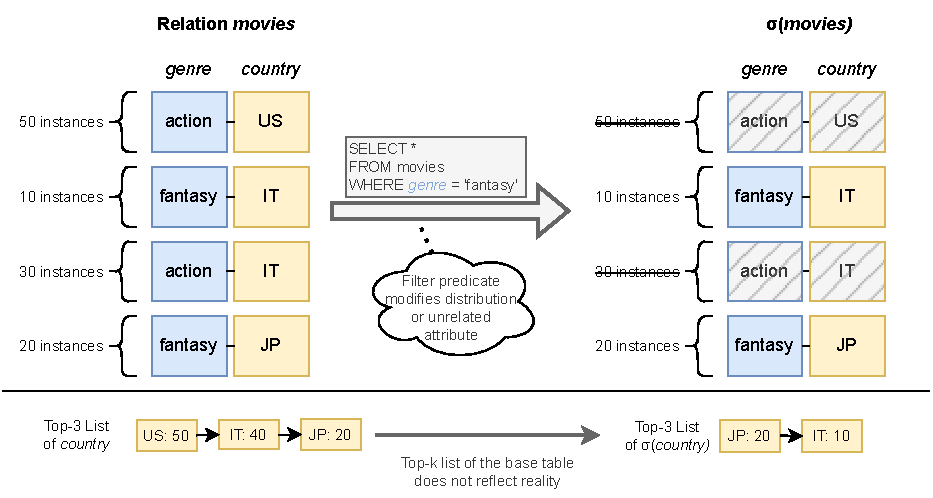
\includegraphics[width=\linewidth]{figures/topk-filters.pdf}
	\caption{Static top-k lists can be misleading in the light of filter predicates.}
	\label{fig:topk-filter-mismatch}
\end{figure}

The main idea of the \emph{approximate bound} is to split the calculation into two parts, i.e. $\text{upper}(R.a = S.b) \coloneqq \text{upper}_\text{top}(R.a = S.b) + \text{upper}_\text{rem}(R.a = S.b)$, where the first bound is directly based on the top-k lists and the second bound accounts for all remaining attribute values with lower frequencies. 
Deriving an upper bound for values in the top-k lists is pretty straightforward: for each value in either top-k list, its frequency is multiplied by the value frequency in the other top-k list, falling back to $f^\ast$ if necessary. 
Thus, $\text{upper}_\text{top}$ can be expressed as

\begin{definition}[Top-k based approximate upper bound]
    \begin{equation}
        \text{upper}_\text{top}(R.a = S.b) \coloneqq \sum_{a \in R.a} AF_R(a) \cdot AF_S(a)\:+\sum_{b \in S.b \setminus R.a} AF_R(b) \cdot AF_S(b)
    \end{equation}
    \label{def:approx-bound-topk}
\end{definition}



Deriving an upper bound for all remaining attribute values is significantly harder: Although in principle the UES formula can be used to estimate the maximum cardinality of two attribute sets based on their maximum frequency, some of these values might have already been processed as part of $\text{upper}_\text{top}$. 
Thus, these values should not be considered again in the remaining bound. 
At the same time, frequencies from the top-k lists cannot simply be used to ``initialize'' the remaining values, due to a fundamental disconnect between the top-k list of an attribute \sql{R.a} and the attribute instances that are actually available during query execution: while top-k lists are computed for all attribute values in a base table, at query runtime, the distribution and count of these attribute value instances may be changed fundamentally after applying filter predicates on the base tables. 
Consider Fig.~\ref{fig:topk-filter-mismatch}: the filter predicate completely removes the most frequent value and changes the order of the remaining two attribute values. 
Since the filter predicate can be entirely independent from the attribute being joined, the top-k list can only be considered as a static upper bound of the true attribute frequencies.
Since there is no direct way to determine which attribute instances are actually available after executing the filter predicate as long as only basic statistics are considered, we make the pessimistic assumption that none of the values from the top-k list are actually available and the remaining values lie entirely in the scope of $\text{upper}_\text{rem}$.
Thus, the $\text{upper}_\text{rem}$ bound becomes a full UES bound based on the maximum remaining frequency, i.e. $f^\ast$:

\begin{definition}[Remaining UES bound of the approximate top-k bound]
    \begin{equation}
        \text{upper}_\text{rem}(R.a = S.b) \coloneqq \min \biggl( \frac{|\sigma(R)|}{f^\ast_R}, \frac{|\sigma(S)|}{f^\ast_S} \biggr) \cdot f^\ast_R \cdot f^\ast_S
    \end{equation}
    \label{def:approx-bound-remainder}
\end{definition}

\begin{figure}[tb]
	\centering
	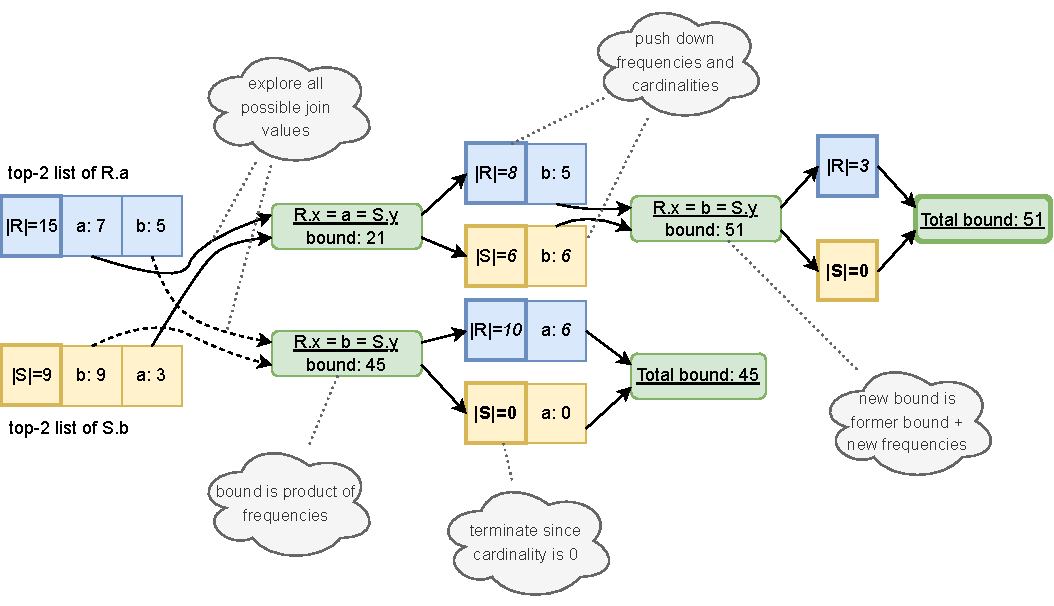
\includegraphics[width=\linewidth]{figures/top-k-estimation-cautious.pdf}
	\caption{Join cardinality estimation using the cautious top-k bound.}
	\label{fig:topk-formula-cautious}
\end{figure}

The issue of top-k lists that are unrelated to the attribute instances is actually also present when calculating the $\text{upper}_\text{top}$ bound: the processed frequencies can significantly overestimate the number of tuples that are truly available. 
However, in this case, we know the total number of available tuples as well as the number of processed tuples per relation. 
Thus, we can slightly mitigate the impact of overestimation by constructing an adjustment factor for \sql{R} as well as for \sql{S}. 
Each factor is simply the ratio between available tuples and processed tuples. 
The factors will be applied as soon as they are smaller than 1 (i.e. there was an overestimation). 
Strictly speaking, this trick assumes a uniform distribution of the overestimation, i.e. that each attribute value is overestimated by the same fixed delta. 
This may drop the upper bound for the top-k list below the actual cardinality in some rare cases. 
By applying the $\text{upper}_\text{rem}$ bound as defensively as presented in Definition~\ref{def:approx-bound-remainder}, this issue is largely mitigated, leaving the bound \emph{effectively} as an upper bound. 
Still, there may be situations where the overestimation via $\text{upper}_\text{rem}$ is not enough to compensate the underestimation caused by the adjustment factors, hence the name of an \emph{approximate} upper bound.

\subsection{Cautious Top-k Bound}
\label{sec:tighter-bounds-cautious}

The approximate nature of the previous bound motivates research in an entirely different direction. 
The \emph{cautious top-k bound} iteratively tries to construct the maximum number of join tuples based on the entries in the top-k lists and the total number of available tuples. A pseudo-code implementation of this strategy is given in Algorithm~\ref{alg:cautious-topk-bound} and illustrated in Fig.~\ref{fig:topk-formula-cautious} (branches and decisions of the algorithm are depicted in green):

\begin{algorithm}[tb]
    \caption{Pseudo-code implementation of the cautious top-k bound.}
    \label{alg:cautious-topk-bound}
    \begin{algorithmic}[1]
        \Function{cautious bound}{top(R), top(S), |R|, |S|, current bound}
            \If{|R| = 0 or |S| = 0}
                \State \Return current bound
            \EndIf
            \If{top(R) is empty and top(S) is empty}
                \State calculate UES bound based on $f^*$ and remaining tuples counts
                \State \Return current bound + UES bound
            \EndIf
            \ForAll{attribute values $v$ in top(R) and top(S)}
                \State $candidate \gets AF_R(v) \cdot AF_S(v)$
                \State $|R'| \gets max(|R| - AF_R(v), 0)$ \Comment adjust the remaining tuples
                \State $|S'| \gets max(|S| - AF_S(v), 0)$
                \State limit top(R') frequencies and $f^\ast_R$ to |R'| \Comment top(R') $\coloneqq$ top(R) $\setminus\:v$
                \State limit top(S') frequencies and $f^\ast_S$ to |S'| \Comment $f_i' = min(f_i, |R'|)$
                \State value bound $\gets candidate\:+\:$ cautious bound(top(R'), top(S'), |R'|, |S'|, current bound) 
            \EndFor
            \State \Return current bound + maximum value bound
        \EndFunction
    \end{algorithmic}
\end{algorithm}

In each iteration, the cautious top-k bound tries to obtain the maximum possible bound given its current state. 
This is achieved by systematically simulating the number of outgoing tuples for each attribute value in the top-k lists. In Fig.~\ref{fig:topk-formula-cautious}, this initially means exploring the attribute values $a$ and $b$.
For each value, the size of its partial join result is calculated (line 8) and included in the upper bound. 
Afterwards, the top-k lists as well as the total number of available tuples are adjusted based on the value that was just ``consumed'' (lines 9 to 12). 
To adjust the total number of tuples available for each relation, the value's frequency is simply subtracted from the current count. 
Top-k lists are updated to no longer include the candidate value and each frequency including $f^\ast$ is enforced to be at most as large as the remaining number of tuples. In Fig.~\ref{fig:topk-formula-cautious}, the top-k lists contain just 1 more value after the first selection.
At this point, the maximum bound for the smaller top-k lists can be calculated (line 13), leading to a recursive structure. 
Recursion terminates if either no more tuples are available (line 2), or the top-k lists are empty (line 4). 
In the first case, both relations have been consumed completely and the current bound is the maximum bound for this branch. 
In the second case, the remaining values are estimated using the UES bound. 
Once the bound for all candidate values has been determined, the algorithm selects the maximum possible bound and calculates the final bound (line 14).

This strategy effectively determines the upper bound for each permutation of attribute value instances and thus suffers from a large computational complexity if implemented naively.
However, a more elaborate implementation can effectively prune large parts of the search space by checking, whether the largest possible bound still contained in the top-k lists can exceed the maximum bound already observed. If this is not the case, there is no point in further exploring the current branch. Furthermore, many bounds of intermediate joins can be re-used if the top-k lists of their recursion branches are equal. For example, if a bound has been calculated for join $A \bowtie B \bowtie C \bowtie D$ and join $A \bowtie B \bowtie D \bowtie C$ is explored, the previous results could potentially be re-used.
Additional optimization techniques for an efficient implementation should be explored in future research.

\subsection{Updating Top-k Based Statistics for $n$-way Joins}
\label{sec:tighter-bounds-stats}

\begin{figure}[tb]
	\centering
	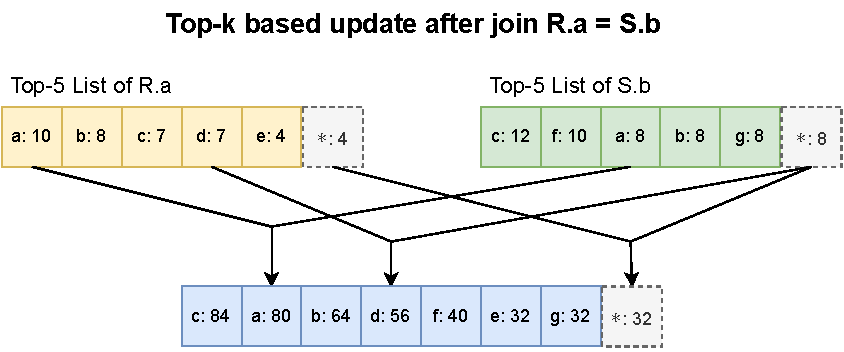
\includegraphics[width=0.8\linewidth]{figures/top-k-update.pdf}
	\caption{Merging two top-k lists after a join.}
	\label{fig:topk-update-merge}
\end{figure}

Besides the calculation of the upper bounds themselves, the underlying data structures also have to be updated to estimate higher-order joins that involve 3 or more relations. 
In the case of top-k lists, this issue is twofold: First, the top-k lists of the join attributes have to be combined, integrating the knowledge of both individual lists. 
This problem can be solved in a straightforward manner: The resulting top-k list contains the sum of both source frequencies for each value in either top-k list, again falling back to the $f^\ast$ frequencies as necessary (Fig.~\ref{fig:topk-update-merge}). 
The $f^\ast$ frequency of the merged top-k list can likewise be estimated as the product of both source $f^\ast$ frequencies. 
The second case is the update of a top-k list that is not directly involved in the join (a \emph{third-party list}). 
This process is especially important since that list may take part in a later join and the associated frequencies must therefore reflect the current state of the intermediate join result. 
The fundamental problem for this update is the lack of correlation information between the joined top-k list and the third-party list. 
For an upper bound-driven approach, this demands another pessimistic assumption: In the worst case, each entry in the third-party list could correlate entirely with the maximum frequency of the joined top-k list. 
Thus, the maximum possible frequency of each updated value in the third-party list is the product of its current frequency and the maximum frequency in the joined top-k list. 
In general, this strategy will heavily overestimate the frequencies in the updated top-k list, but without additional information or simplifying assumptions it is not possible to figure out how much each frequency has been overestimated. 
This matches the basic maximum frequency update of UES and generalizes that idea to top-k lists.

\section{Evaluation}
\label{sec:Eval}

We focus our evaluation on two major aspects of \emph{PostBOUND}: On the one hand, we examine the independence of \emph{PostBOUND} from specific workloads using two well-known benchmarks and different PostgreSQL versions.
On the other hand, we explore the potential of upper bound-driven query optimization in more detail.
This includes (i) the computed join orders, (ii) the generation of subqueries, (iii) the effect of tighter upper bounds, and (iv) the potential of the selection of physical operators.
Generally, all experiments are executed on an Ubuntu 20.04 machine with an Intel i7-6700 HQ processor, 32 GB of main memory and an SSD storage.
Unless stated otherwise, we run the benchmarks on PostgreSQL 14.

%\subsection{Analyzing UES: Join Orders and Subquery Generation}
%\label{sec:eval-postbound}


\textbf{Analyzing UES - Join Orders:}
To analyze \emph{PostBOUND}'s applicability to different database schemas and workloads, we examine the Join-Order-Benchmark (JOB)~\cite{DBLP:journals/pvldb/LeisGMBK015} as well as the Star-Schema-Benchmark (SSB)~\cite{DBLP:journals/corr/Sanchez16a}.
Queries of the JOB are optimized with UES using the precise base table estimation and defensive subquery generation strategies (cf. Section~\ref{sec:postbound-join-ordering}).
Precise base table estimation allows for the best reproducibility of the optimized queries, since the estimates are derived directly from the live database.
Moreover, the defensive subquery generation was also used in \cite{hertzschuch-21-ues}, enabling better comparability with these results.
The queries of the SSB are optimized based on the base table estimates of the native PostgreSQL optimizer to demonstrate this functionality.
The underlying TPC-H database is setup to use a scale factor of $1$.
In addition to different benchmarks, we also evaluate both workloads on two versions of PostgreSQL: v12.4 was already used in \cite{hertzschuch-21-ues} and v14.2 was the latest release of PostgreSQL at the time initial work on \emph{PostBOUND} began. Table~\ref{tab:postbound-benchmarks} contains the total runtime for each benchmark setting.
Native optimization in this context means optimization by the built-in optimizer of PostgreSQL, but without usage of nested loop joins.
This constraint matches a similar requirement by UES and enables us to focus on the join order, rather than the operator selection, which is beyond the scope of original UES.

\input{table-01}

The JOB benchmark results highlight two interesting insights: On the one hand, both PostgreSQL versions show a much better performance of UES compared to the native optimizer.
This basically confirms the results presented in \cite{hertzschuch-21-ues}.
On the other hand, nearly the entire speedup of UES on both PostgreSQL versions is caused by two queries with catastrophic join orders. In the case of Postgres v14.2, these queries are  8c and 19d. Each of these queries is running more than 200 seconds faster when optimized with UES. Execution of the UES variants takes less than 10 seconds, which demonstrates the disastrous effects bad join orderings can have. However, some queries are also slowed down by UES, although to a much smaller degree. For example, query 7c is slowed down the most by about 4 seconds.
Results on SSB are much more similar, which is mostly caused by the much smaller data set. However, the runtimes show that the UES optimized queries are neither significantly better, nor significantly worse than native optimization.
Nonetheless, the overall simpler queries of the SSB also stray away from the primary focus of upper bound-driven query optimization, which is intended for complex queries with many joins and complicated filter predicates.

\begin{figure}[tb]
	\centering
	\begin{subfigure}[b]{0.47\textwidth}
	    \centering
	    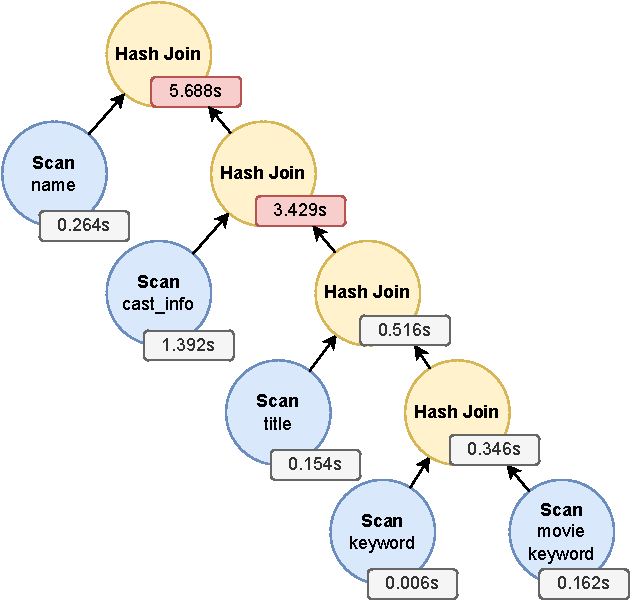
\includegraphics[width=0.8\textwidth]{figures/subquery-example-job-6c-linear.pdf}
	    \caption{Linear execution plan.}
	    \label{fig:subquery-results-linear}
	\end{subfigure}
	\begin{subfigure}[b]{0.47\textwidth}
	    \centering
	    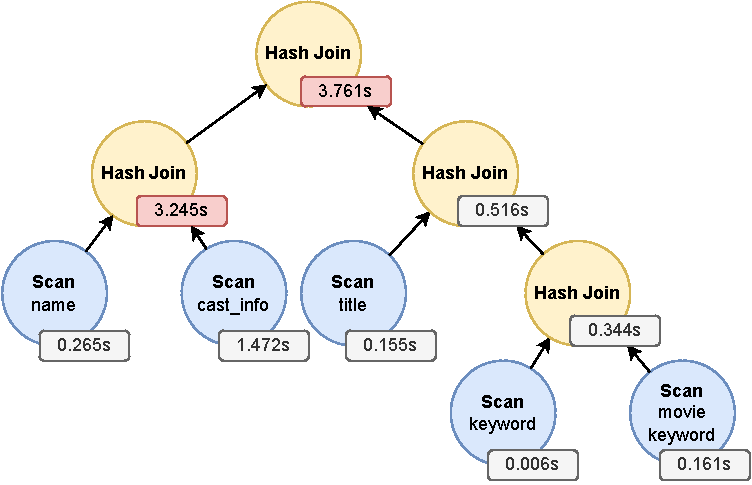
\includegraphics[width=\textwidth]{figures/subquery-example-job-6c-subqueries.pdf}
	    \caption{Bushy execution plan}
	    \label{fig:subquery-results-bushy}
	\end{subfigure}
	\caption{Generating subqueries for JOB query 6c can improve performance substantially.}
	\label{fig:subquery-results}
\end{figure}

\textbf{Analyzing UES - Subquery Generation:}
A central idea of UES is the evaluation of primary key/foreign key joins in subqueries to achieve an up-front reduction of the foreign key cardinality.
However, introducing subqueries also implies additional pipeline breakers when executing the query in PostgreSQL.
Thus, we investigate the impact of subqueries on individual queries next by optimizing the JOB workload with two UES settings: The first one uses the smart subquery generation strategy while the second setting produces entirely linear queries.
Based on this setup, for example, query 6c shows the largest speedup of about 33\% (5.7s to 3.8s) when using subqueries.
The resulting execution plans for both settings are sketched in Fig.~\ref{fig:subquery-results}: executing the join between \sql{name} and \sql{cast\_info} as a subquery not only reduces the number of processed tuples, but also allows for a parallel processing of that join.
Nevertheless, subqueries do not always lead to a performance benefit.
In fact, query 7a is slowed down the most with about 0.6 seconds (13\% of the linear runtime).
Thus, it is important to create subqueries carefully and a smart generation policy -- e.g. based on tight upper bounds -- seems to work well in these cases.

%\subsection{Advancing UES: Tighter bounds and physical operators}
%\label{sec:eval-tighter-bounds}


\textbf{Advancing UES - Tighter Upper Bounds:}
Tight upper bounds have been proposed as a potential solution for many problems in this paper.
In this section, we evaluate how large the impact of the cautious and approximate algorithms presented in Section~\ref{sec:TighterBounds} already is.
For this, we vary the length of the top-k lists for both algorithms and compare the results to a UES baseline.
In all cases, the JOB queries are upper bound-driven optimized using precise base table estimates and the smart subquery generation policy.

Looking at the median upper bounds across all JOB queries in Fig.~\ref{fig:results-topk-upper-bounds} indeed reveals a substantial improvement of the bounds as the top-k lists become longer.
In fact, using top-500 lists achieves a maximum improvement of factor 210,000 compared to the UES bound.
Although this is an extreme case, many upper bounds still improve several orders of magnitude when using top-k lists with just 50 or 100 attribute values.
For shorter top-k lists, the improvement is much smaller, as is expected.
This is caused by two main factors: shorter lists allow for fewer actual matches of attribute values, causing more usage of the $f^\ast$ frequencies.
At the same time, shorter lists also allow for less drop-off of frequencies, again resulting in values that are closer to the UES bound.

\begin{figure}[tb]
	\centering
	\begin{subfigure}[b]{0.47\textwidth}
	    \centering
	    \includegraphics[width=\textwidth]{figures/plot-job-upper-bounds.pdf}
	    \caption{Final bounds of each query.}
	    \label{fig:results-topk-upper-bounds}
	\end{subfigure}
	\begin{subfigure}[b]{0.47\textwidth}
	    \centering
	    \includegraphics[width=\textwidth]{figures/plot-job-optimization-time.pdf}
	    \caption{Optimization time of the workloads.}
	    \label{fig:results-topk-optimization-time}
	\end{subfigure}
	\caption{Impact of the top-k based bound estimation on the JOB queries.}
	\label{fig:results-topk}
\end{figure}

A central advantage of the approximate formula becomes apparent when looking at the optimization time in Fig.~\ref{fig:results-topk-optimization-time}: It stays very low at a maximum of 3 seconds for all queries in the JOB.
This is a sharp contrast to the cautious formula, which takes over 1 minute of optimization time already at top-5 lists.
This increase in optimization time is also the reason why larger top-k lists are not optimized with the naive implementation of the algorithm.
Despite the smaller bounds, only a few join orders are actually updated.
In fact, the cautious algorithm only updates 5 queries across all settings.
Although this number becomes slightly larger with 31 queries for the approximate formula, it is still quite small considering the 113 queries that are executed.
This indicates that UES is sufficient for many queries and that more elaborate algorithms are required to close in on the estimates of the native optimizer.
The few updated queries also lead to very little change of the overall workload runtime.
Across all settings, the maximum deviation from UES is about 10 seconds, which is almost negligible considering the complexity of the workload and its overall duration.
Even though the evaluated formulas are prototypes by nature, they still achieve a considerable improvement in terms of their upper bounds.
This motivates further research in that direction and especially the application of the bounds for different tasks.


\textbf{Advancing UES - Physical Operator Selection:}
Besides the generation of optimized join orders, \emph{PostBOUND} also enables the selection of physical operators (cf. Section~\ref{sec:postbound-operator-selection}), thereby removing the restriction to hash joins normally imposed by UES.
A natural application of the operator selection is to further exploit the performance gains enabled by subqueries.
Since these queries are by design joins between a primary key and a foreign key table, they can be implemented more efficiently using index-nested loop joins.
Thus, we again optimize the JOB workload using UES and the smart subquery generation policy.
For each resulting subquery, we use \emph{PostBOUND} to generate query hints that enforce the execution of that subquery as an index-nested loop join. Fig.~\ref{fig:idxnlj-results} shows the final execution plan for query 8d, which is improved the most by this strategy.
Primary key filters are shown in yellow boxes while tables that are n:m joined appear in blue.
Each join is annotated by its operator, as well as the point in time when it is executed.
The subquery \sql{cast\_info $\bowtie$ role\_type} is executed as an index-nested loop join in parallel to the join \sql{aka\_name $\bowtie$ name}.
The choice of operators results in a 45\% speedup (5.7s to 2.6s) compared to a pure hash join-based execution.
This simple strategy barely scratches the surface of elaborate techniques for physical operator selection, it focuses exclusively on joins between base tables within subqueries and does not consider the upper bounds associated with each join at all.
Advanced approaches such as TONIC~\cite{DBLP:journals/pvldb/HertzschuchHHL22} could perform much better.
Still, the simple strategy of executing all subqueries as index-nested loop joins already shows the potential of appropriate operator choice that can be explored in future work.

\begin{figure}[tb]
	\centering
	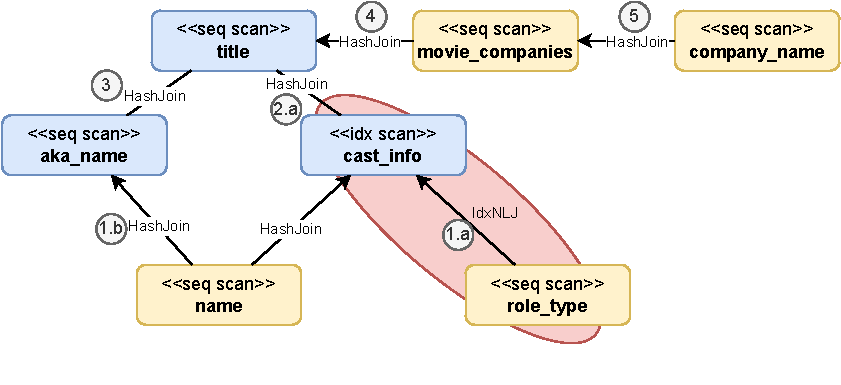
\includegraphics[width=0.95\linewidth]{figures/idxnlj-example-job-8d.pdf}
	\caption{Join order and operator selection for JOB query 8d. Subqueries use Index-NLJ hints.}
	\label{fig:idxnlj-results}
\end{figure}

\section{Related Work}
\label{sec:RealtedWork}

Generally, the optimization of SPJ queries entails two major challenges: (i) finding a good join order and (ii) selecting the best-fitting physical join operator for each single join within the chosen join order. 
According to~\cite{DBLP:conf/pods/Chaudhuri98}, to solve both challenges, state-of-the-art SPJ query optimizer require precise estimates of intermediate join result sizes (cardinalities). 
Unfortunately, as shown in~\cite{DBLP:conf/icde/PerronSKS19}, ad-hoc estimation techniques are unlikely to achieve such precise estimates. 
Additionally, Leis et al.~\cite{DBLP:journals/pvldb/LeisGMBK015} provide empirical evidence that cost-based optimizers are prone to disastrous planning decisions if precise cardinality estimates cannot be provided. 
To tackle this issue, recent work investigates more computationally intensive sketches~\cite{DBLP:conf/sigmod/CaiBS19,DBLP:conf/sigmod/IzenovDRS21,DBLP:conf/sigmod/KipfVMKRLB0K19} or machine learning (ML) approaches~\cite{DBLP:journals/pvldb/HilprechtSKMKB20,DBLP:conf/cidr/KipfKRLBK19,DBLP:journals/pvldb/NegiMKMTKA21,DBLP:conf/sigmod/WoltmannHTHL19,DBLP:journals/pvldb/YangKLLDCS20} to achieve precise cardinality estimates. 
Beyond cardinality estimation, some ML approach apply reinforcement learning (RL) for holistic query plan optimization~\cite{DBLP:journals/corr/abs-1808-03196,DBLP:conf/sigmod/MarcusNMTAK21,DBLP:journals/pvldb/MarcusNMZAKPT19}. 
For example, Bao~\cite{DBLP:conf/sigmod/MarcusNMTAK21} learns and injects SQL hints to guide general planning decisions of the underlying optimizer. 

An alternative approach to precise cardinality estimates is to compute an upper bound for each intermediate result. 
This approach originated in the database theory community~\cite{DBLP:conf/soda/GroheM06}.
Atserias et al.~\cite{DBLP:conf/focs/AtseriasGM08} introduced a smart formula -- nowadays called the AGM bound -- that gives a tight upper bound on the query result in terms of the cardinalities of the input tables. 
This upper bound was improved by the \emph{polymatroid bound}, which takes into account both the cardinalities, and the degree constraints as well as including functional dependencies as a special case~\cite{DBLP:journals/jacm/GottlobLVV12,DBLP:conf/pods/KhamisNS16,DBLP:conf/pods/000118}.
Fundamentally, an upper bound could be used by any cost-based query optimizer in lieu of precise cardinality estimates and this idea was recently pursued by the database systems community, where the upper bound appears under various names such as bound sketch, cardinality bound, or pessimistic cardinality estimator~\cite{DBLP:conf/sigmod/CaiBS19,DBLP:journals/corr/abs-2201-04166,hertzschuch-21-ues}. 
For example, Cai et al.~\cite{DBLP:conf/sigmod/CaiBS19} introduced a pessimistic cardinality estimator, which uses Count-Min sketches for capturing join crossing correlations. 
The sketch building process introduces significant overhead when the number of join increases.
In contrast to that, our UES concept~\cite{hertzschuch-21-ues} maintains the pessimistic property for cardinality estimation while replacing sketches with a simple formula based on available basic statistics (most frequent attribute values). 
With \emph{PostBOUND}, we presented a comprehensive framework for all these upper bound approaches in PostgreSQL consisting of two separate components as described in Section~\ref{sec:PostBound}.
Each component focuses on a single challenge for SPJ query optimization, namely finding a good join order and selecting the best-fitting physical operator.
Moreover, we introduced and evaluated ideas to improve our simple formula on basic statistics -- top-k lists -- to tighten the upper bound.
In this context, the main challenge is to find upper bound approaches whose computational cost is low. 
\section{Conclusion}
\label{sec:Conclusion}
The optimization of arbitrary select-project-join (SPJ) queries is still an active research topic.
In this context, deriving the necessary cardinality estimates from upper bounds is a promising strategy.
To foster research in that direction, we have introduced \emph{PostBOUND}, a generalized framework implementation to seamlessly integrate upper bound SPJ query optimization in PostgreSQL. 
\emph{PostBOUND} provides abstractions to integrate arbitrary upper bounds, to model joins required by an SPJ query and to iteratively construct an optimized join order. Other than calculating the join order, \emph{PostBOUND} also enables the selection of physical operators, and can thus mimic the entire query optimization process.
To highlight the extensibility of \emph{PostBOUND} and to show the research potential, we have additionally presented two tighter upper bound variant ideas using top-k statistics in this paper.
Our evaluation has shown the efficiency and broad applicability of \emph{PostBOUND} on different workloads and using different PostgreSQL versions. 
Moreover, we have also highlighted the impact of the proposed tighter upper bound variants. 

%%% Angabe der .bib-Datei (ohne Endung) / State .bib file (for BibTeX usage)
\bibliography{references} %\printbibliography if you use biblatex/Biber
\end{document}
